
%(BEGIN_QUESTION)
% Copyright 2011, Tony R. Kuphaldt, released under the Creative Commons Attribution License (v 1.0)
% This means you may do almost anything with this work of mine, so long as you give me proper credit

En svært nyttig egenskap ved en ``smart'' ventilposisjoner er muligheten til å måle og plotte sammenhengen mellom ventilspindelens posisjon og lufttrykket i aktuatoren. Skisser hvordan en ``frisk'' {\it ventilsignatur} bør se ut, gitt en ventil med følgende egenskaper:

$$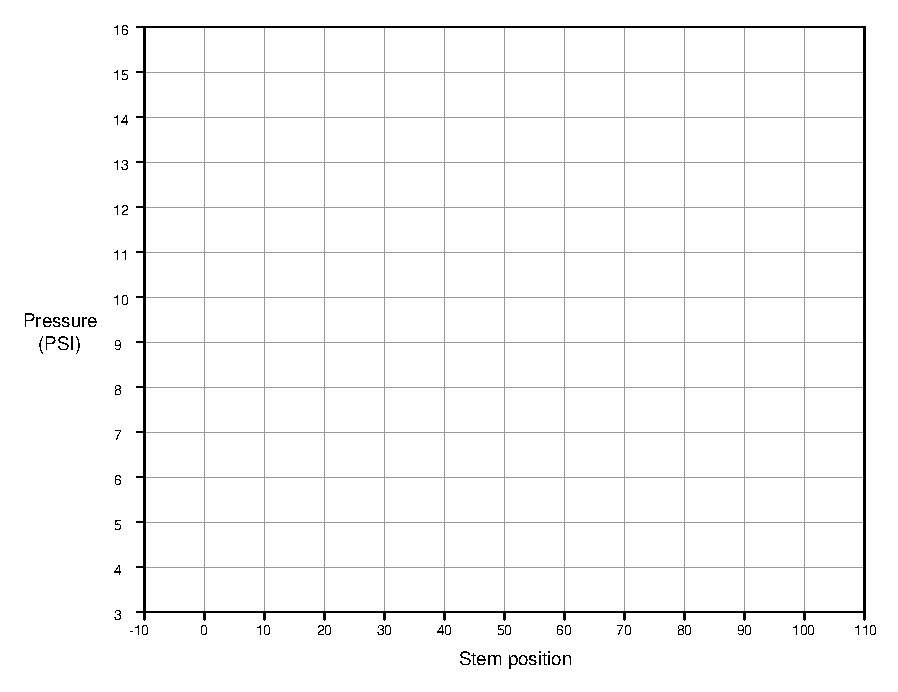
\includegraphics[width=15.5cm]{i01539x01.eps}$$

\begin{itemize}
\item{} Globe-trim med spindelføring
\vskip 10pt
\item{} Reversvirkende pneumatisk aktuator
\vskip 10pt
\item{} Direktevirkende ventilhus
\vskip 10pt
\item{} Likeprosentlig trimkarakteristikk
\vskip 10pt
\item{} 6 PSI nedre bench-set-trykk
\vskip 10pt
\item{} 15 PSI øvre bench-set-trykk (slutt av slag)
\end{itemize}

\vskip 20pt \vbox{\hrule \hbox{\strut \vrule{} {\bf Forslag til sokratisk diskusjon} \vrule} \hrule}

\begin{itemize}
\item{} Identifiser noen reguleringsventilproblemer som kan diagnostiseres ved dyktig tolkning av et ventilsignatur-plot.
\end{itemize}

\underbar{file i01539}
%(END_QUESTION)





%(BEGIN_ANSWER)


%(END_ANSWER)





%(BEGIN_NOTES)

Denne ventilsignaturen er {\it ideell}, og viser ingen friksjon i det hele tatt:

$$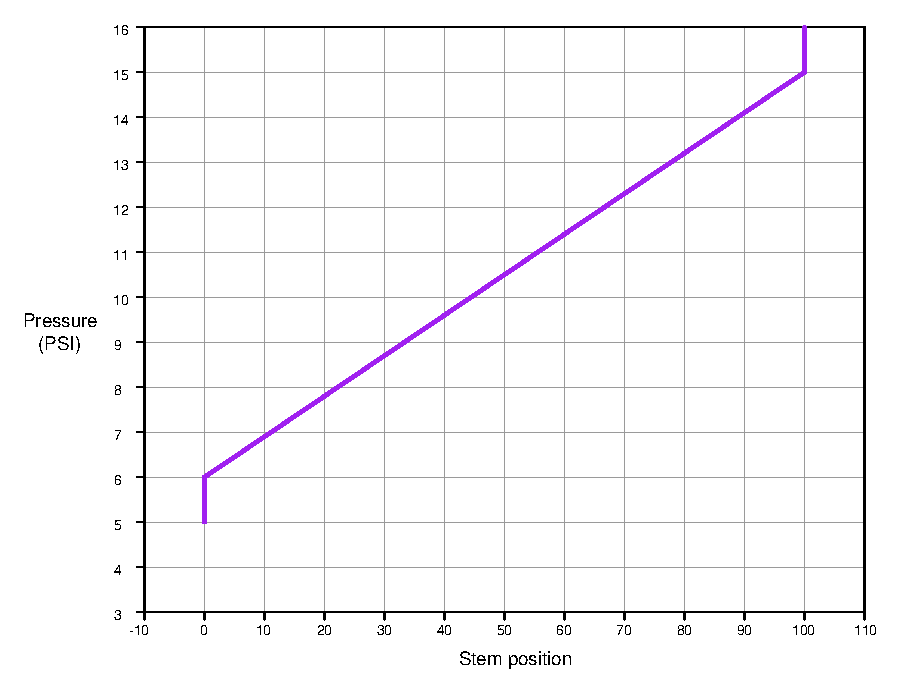
\includegraphics[width=15.5cm]{i01539x02.eps}$$

At trimmen er likeprosentlig er irrelevant informasjon, men det kan få noen studenter til å forsøke å skissere ventilsignaturen som en {\it kurve}. At denne ventilen er spindelført påvirker heller ikke signaturen.

Teknisk sett er det relevant at ventilhuset er direktevirkende, fordi det forteller hvor {\it seteprofilen} finnes på denne ventilen. Den grove ventilsignaturen jeg viser, gir imidlertid ikke dette detaljnivået, så vi kan si at ventilhusets virkemåte er irrelevant innenfor rammen av denne oppgaven.



\vskip 20pt \vbox{\hrule \hbox{\strut \vrule{} {\bf Forslag til sokratisk diskusjon} \vrule} \hrule}

\begin{itemize}
\item{} Forklar hvorfor det ville være feil å skissere denne funksjonen som en kurve i et forsøk på å reflektere likeprosentlig ventilkarakteristikk.
\end{itemize}

%INDEX% Final Control Elements, valve: diagnostic signature for pneumatic actuator

%(END_NOTES)

